\chapter{Monte Carlo Models of Signal and Background} \label{ch:monte_carlo}

\section{Signal Modeling}\label{sec:signal_modeling}

Simulated gluino pair-production events were generated for use in the analysis.
Separate samples were generated for the direct decay and cascade decay models described in~\ref{subsec:rpv_gluino}.
For the direct decay model, events were generated for gluino mass ranging from 900~GeV to 1.8~TeV .
For the cascade model, the gluino mass was varied from 750~GeV up to 2.1~TeV, with the neutralino mass ranging from
450~GeV to 1.9~TeV .
For all signal points, $m_{\tilde{g}} > m_{\tilde{\chi}_1^0}$.
Signal events were simulated for a discrete set of mass points.
Figure~\ref{fig:signal_cascade_grid} indicates the $\left(m_{\tilde{g}}, m_{\tilde{\chi}_1^0}\right)$ points for which
signal evens were generated.

\begin{figure}[!ht]
    \centering
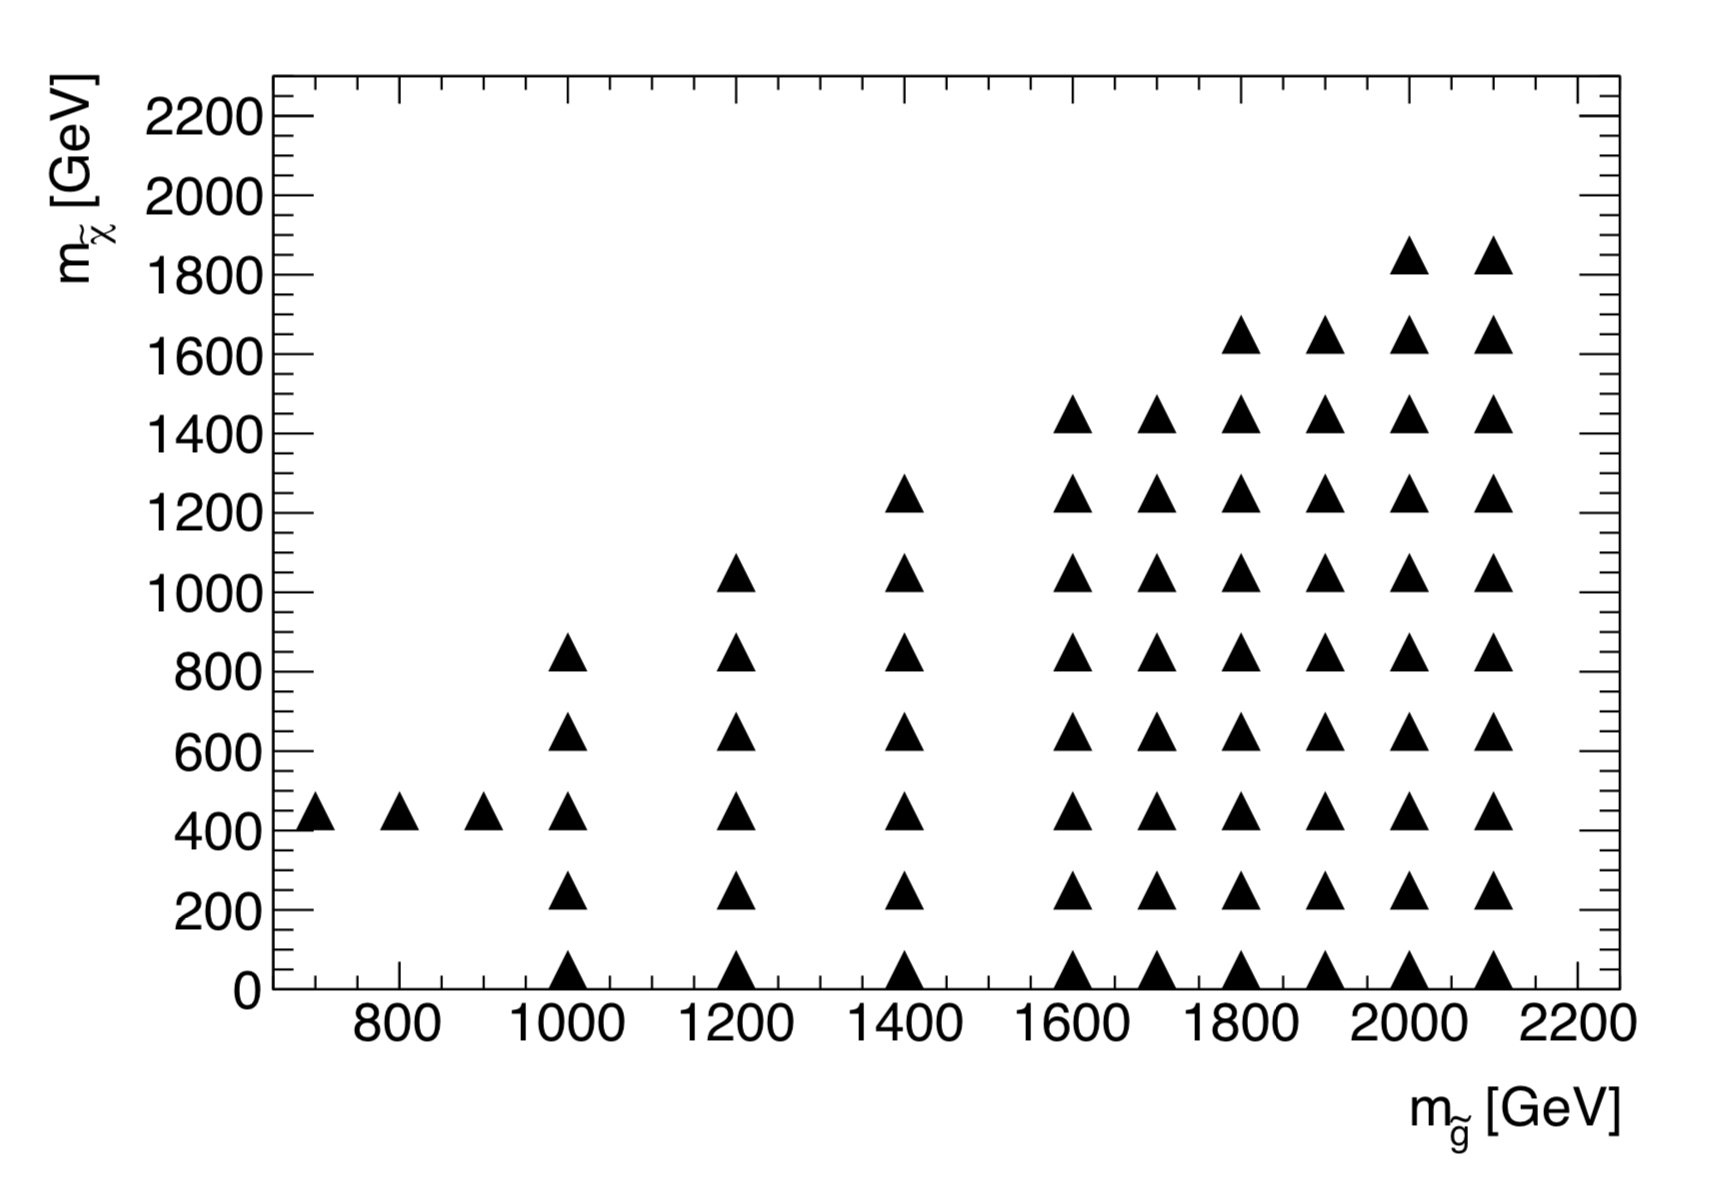
\includegraphics[width=0.8\linewidth]{signal_cascade_grid}
\caption{The grid of gluino and neutralino masses for which simulated cascade decay events were generated. The triangles
indicate the mass points that were generated.}
\label{fig:signal_cascade_grid}
\end{figure}

\subsection{Event generation}\label{subsec:signal_event_gen}

Matrix elements for gluino pair production were generated with \textsc{MadGraph\_aMC@NLO} v2.3.3,
which is a convenient framework for calculating arbitrary matrix elements at up to next-to-leading order (NLO)~\cite{signal-madgraph}.
\textsc{MadGraph} allows the user to specify the theory being used and the values for the free parameters,
and then it constructs and calculates the necessary Feynman diagram.
In this analysis, matrix elements were calculated at leading order (LO).
In the pair-production matrix elements, up two two additional partons were allowed to be produced along with the
gluino pair.

To model the parts of the collision environment described in~\ref{sec:jet_collisions}, such as the underlying event,
parton shower, and fragmentation, \textsc{Pythia} 8.186 is used~\cite{signal-pythia}.

Interfacing \textsc{MadGraph} and \textsc{Pythia} is made possible by a standardized file format known as Les Houches
Event Format (LHEF)~\cite{signal-lhef}.

As discussed in~\ref{sec:jet_collisions}, there are non-perturbative processes that occur in proton-proton collisions,
which cannot be directly calculated from first principles.
This processes can be parameterized and approximated in a program like \textsc{Pythia},
requiring the creation of several free parameters whose values have to be inferred from data.
The process of inferring these parameters so that the calculations match the data is known as tuning.
For this analysis the A14 set of tuned parameter values were used for modeling the underlying event in
\textsc{Pythia}~\cite{signal-pythia-a14,signal-pythia-tunes}.

The parton distribution functions (PDFs) used for the simulated signal generation are from the NNPDF2.3LO
set~\cite{signal-nnpdf}.

\subsection{Cross-section}\label{subsec:signal_cross_section}
In order to estimate the expected signal yield and uncertainty, the nominal production cross section and its uncertainty
must be known.
Gluino pair-production cross-sections have been calculated at a range of center-of-mass energies, and the results
are summarized in~\cite{signal-xsec}.
The gluino pair-production cross-section and its uncertainty over a range of gluino masses can be seen in~\ref{fig:signal_xsec}.

\begin{figure}[!ht]
    \centering
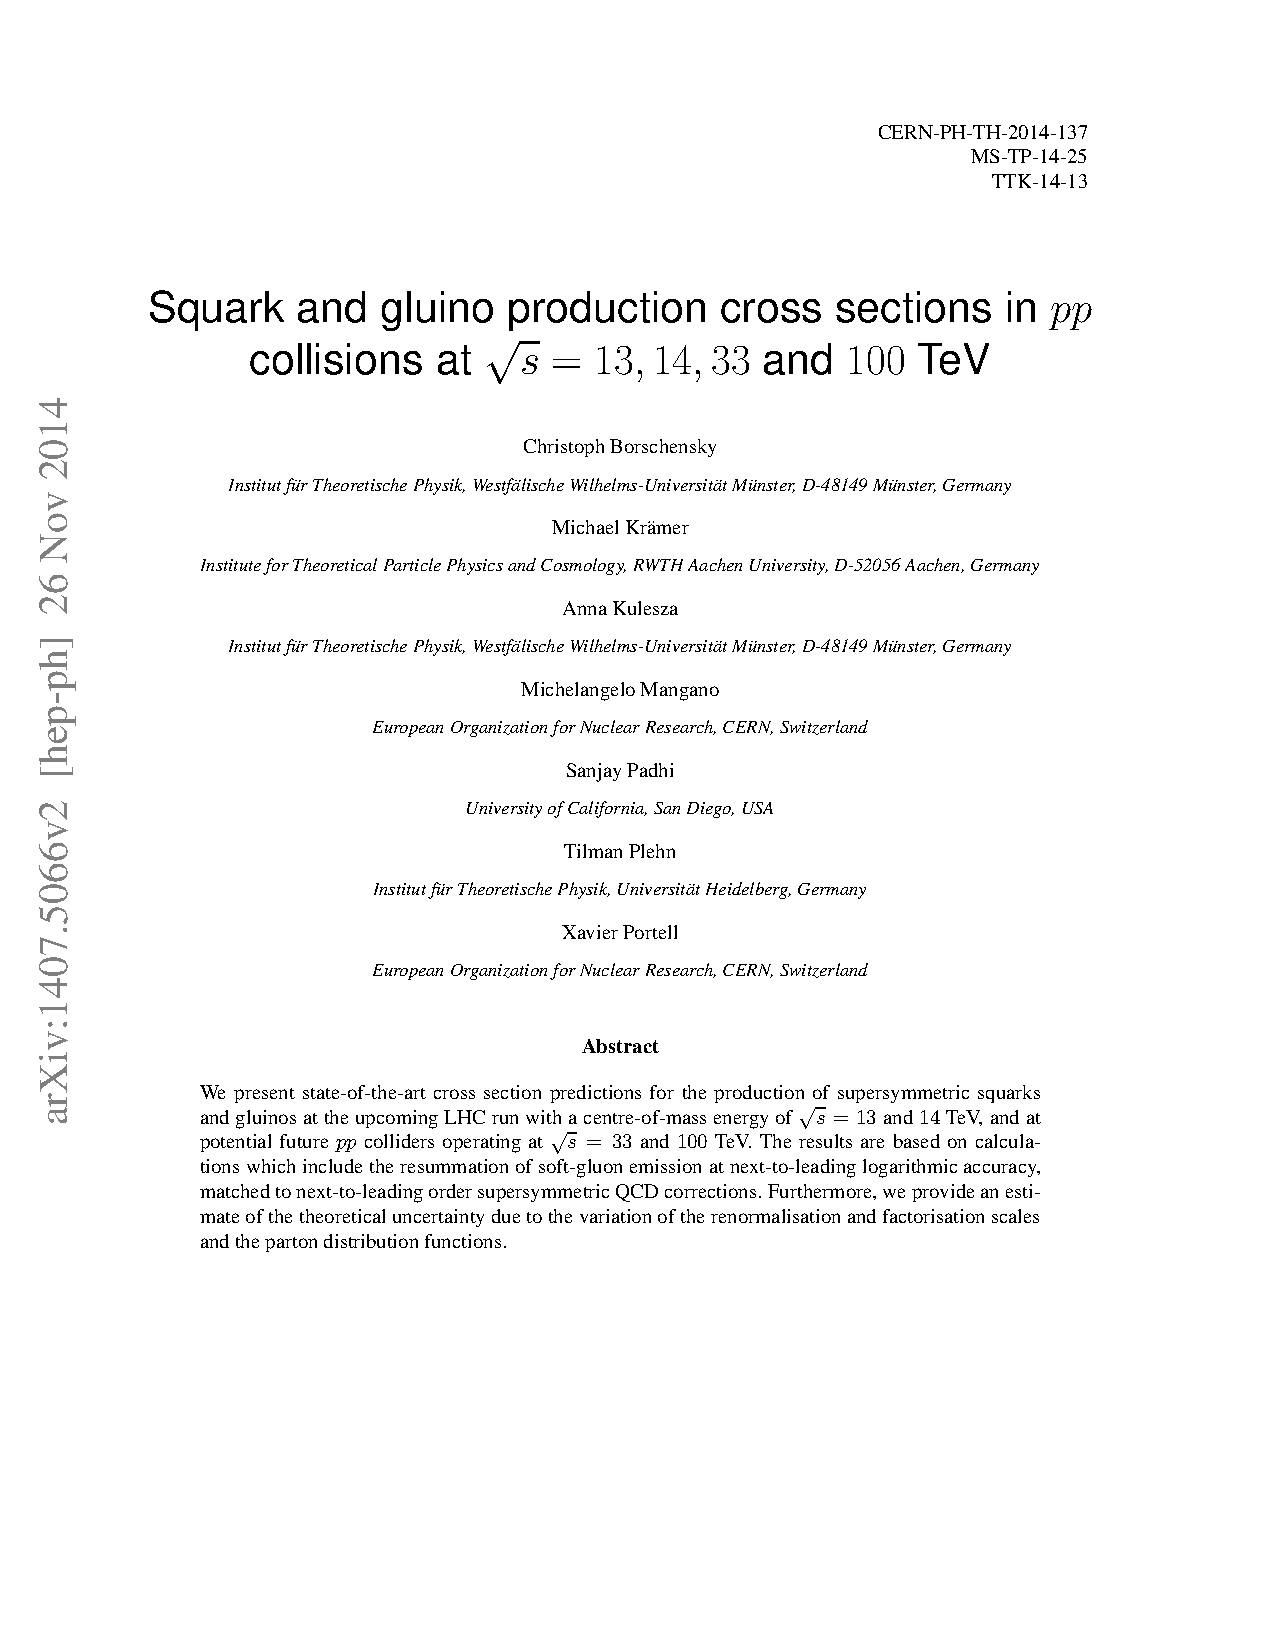
\includegraphics[width=0.8\linewidth]{signal_xsec}
\caption{Gluino pair-production cross-section and uncertainty for $\sqrt{13}~TeV$ proton-proton collisions at the LHC,
calculated at NLO+NLL~\cite{signal-xsec}.}
\label{fig:signal_xsec}
\end{figure}

\section{Systematic Uncertainty Evaluation Method}\label{sec:signal_systematics_method}
There are four main components to the systematic uncertainty on the
estimated signal yield.
These components are the large-R jet mass scale (JMS), the small-R b-tagging uncertainty, the Monte Carlo statistical
uncertainty, and the modelling uncertainty, which includes uncertainty
on parton distribution functions (PDFs), QCD scale uncertainty, and
initial state radiation (ISR) modelling uncertainty.

A given systematic is evaluated by varying a nuisance parameter and
determining the percent difference in signal yield between the nominal
distribution and systematically varied distribution.
When a systematic contains multiple components, those components are treated as
uncorrelated, and their contributions are combined in quadrature.

Systematic uncertainties depend on the gluino and neutralino masses
being considered, as well as the decay mode of direct or cascade.
As such, they are evaluated separately at each point in the mass grid.

\subsection{Jet Mass Scale Uncertainty}\label{subsec:signal_jms_uncertainty}
For the JMS uncertainty, there are four components, called the
baseline, modeling, statistical, and tracking components.
These components are derived from the $R_{trk}$ method~\cite{jet-substructure-perf}.
The JMS uncertainty is largest for $m_{\tilde{g}}=1.0~TeV$, at $\approx 24\%$, and drops to $\approx 8\%$
for signal points with $m_{\tilde{g}}=1.8~TeV$.
It is generally dominated by the tracking uncertainty, followed by the baseline uncertainty.

\subsection{b-Tagging Uncertainty}\label{subsec:signal_btag_uncertainty}
The b-tagging uncertainty is evaluated by varying a set of 25 nuisance parameters.
The result is an uncertainty on the signal efficiency of between $15\%$ and $25\%$.
This uncertainty is only applied to the b-tag signal regions.

\subsection{Monte Carlo Statistical Uncertainty}\label{subsec:signal_mc_uncertainty}
The Monte Carlo statistical uncertainty accounts for the fact that only a limited sample of simulated events are
produced for each mass point.
The uncertainty is derived as $\sigma=\sqrt{\epsilon(1-\epsilon)/N}$, where $\epsilon$ is the
efficiency measured in the sample, and $N$ is the sample size.


\subsection{PDF, QCD scale, and ISR Uncertainties}\label{subsec:signal_qcd_uncertainty}
Evaluating the contribution to the signal efficiency uncertainty from PDF, $\alpha_s$ and ISR modelling uncertainties
requires the generation of truth-level signal simulation samples where different parameters are varied in the generation.

For PDF uncertainties, the internal event weights in the PDF set are varied up and down during the generation.

For the QCD scale uncertainty, the value of $alpha_s$ is varied up and down during the generation.

For ISR uncertainties, the value of the matching scale,v$q_{\textrm{cut}}$ is varied up and down during the generation.

The PDF and QCD scale contributions to the uncertainty are highest at low gluino mass, reaching a maximum of $25\%$ at
$m_{\tilde{g}}=1.0~TeV$, the lowest gluino mass studied.
For higher masses, these uncertainties drop to only a few percent.
